\chapter{Implementación Computacional}

\label{ch:implementation}

\section{Introducción}

En este trabajo, los algoritmos han sido implementados bajo el estándar \CC14 por medio de un conjunto de clases interrelacionadas por herencia y composición. La escalabilidad de las clases permite que cada capa y columna cortical sea generada con la dimensionalidad y el número de unidades deseado. La conectividad entre columnas corticales así como entre capas corticales se genera automáticamente y de manera aleatoria siguiendo la guía de los argumentos pasados a los constructores de los objetos. La implementación computacional está paralelizada con un paradigma híbrido en \gls{mpi}-\gls{omp}.

%The algorithms in this work have been implemented under the standard \CC11 by a set of classes related by inheritance and composition. The scalability of the classes allows every cortical layer and column to be generated with the desired dimensionality and number of units. Connectivity among cortical columns as well as cortical layers is randomly auto-generated with the guide of arguments passed to the object constructors. In order to handle the data produced by the model, a library has been implemented to save the data in Octave/Matlab compatible (.mat) file formats. Every class in the implementation has been parallelized by means of the OpenMP \gls{api}.

\section{Herencia y Estructura Composicional Jerárquica del \glsfirst{el}}

Implementamos nuestros algoritmos con el estándar \CC14 utilizando el paradigma de programación orientada a objetos o \gls{oop} en un conjunto de clases interrelacionadas por herencia y composición. Implementamos conectividad aferente próxima y distante intercolumnar así como los márgenes mínimos/máximos en los pesos sinápticos aferentes en  la clase \glsfirst{el}. Configuramos tal clase como una composición de objetos de la clase \glsfirst{csom}. El miembro principal de la clase \gls{el} es un vector \gls{stl} con objetos \gls{csom}. Un diagrama completo de la estructura composicional y de herencia jerárquica de la implementación se muestra en la Fig. \ref{fig:InheritanceComposition}.

%We implement our algorithms in standard \CC14 using the \gls{oop} paradigm in a set of classes interrelated by inheritance and composition. We implement proximal afferent and distal inter-columnar connectivity   as well as minimum-maximum margins in afferent synaptic weights in the \glsfirst{el} class. We configure such class as a composition of objects of class \glsfirst{csom}. The main member in the \gls{el} class is a \gls{stl} vector of \gls{csom} objects. A complete diagram of the hierarchical inheritance and compositional structure of the implementation can be seen in Fig. \ref{fig:InheritanceComposition}.

\begin{figure}[h!]
    \centering
    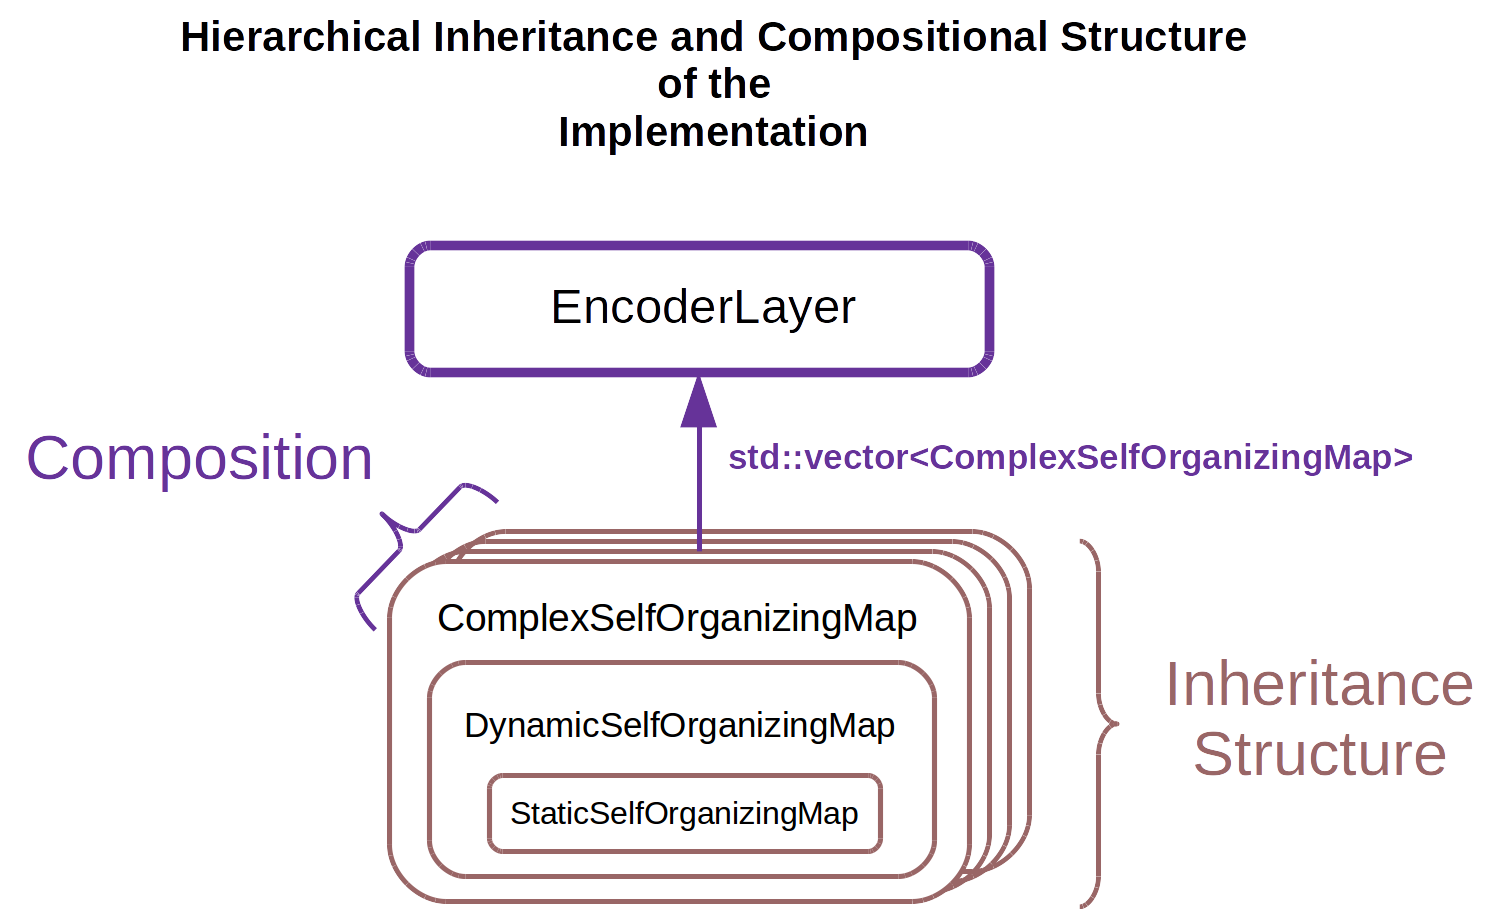
\includegraphics[width=0.8\textwidth]{InheritanceComposition.png}
    \caption{Estructura Hereditaria y Composicional Jerárquica de la implementación del modelo.
    La clase \glsfirst{csom} hereda desde la clase \glsfirst{dsom} la cual hereda desde \glsfirst{ssom}.
    El \glsfirst{el} está formado por la composición de un conjunto de \glspl{csom} agrupados
    en un contenedor std::vector \glsfirst{stl}.}
    %\caption{Hierarchical Inheritance and Compositional Structure of the Model Implementation.
    %\glsfirst{csom} inherits from \glsfirst{dsom} which inherits from \glsfirst{ssom}.
    %The \glsfirst{el} is formed by the composition of a set of \glspl{csom} gathered
    %in a std::vector \glsfirst{stl} container.}
    \label{fig:InheritanceComposition}
\end{figure}















\section{Paralelización del Encoder Layer (EL)}

Paralelizamos la clase \gls{el} por medio del paradigma híbrido \gls{mpi}+\gls{omp}. Distribuimos \glspl{csom} entre \gls{mpi} ranks como un mazo de cartas es distribuido entre diferentes jugadores. Cada \gls{mpi} rank termina con uno o más \glspl{csom} y los \glspl{csom} en cada rank son distribuidos entre diferentes hilos \gls{omp} (Fig. \ref{fig:EncoderParallelization} A y B respectivamente). La información entre \gls{mpi} ranks debe ser transferida en cada paso temporal. Reunimos toda la información correspondiente a los \glspl{csom} en cada rank y luego utilizamos la función \gls{mpi} Bcast  para transmitir tal información utilizando un protocolo de comunicación especial por medio del cual especificamos los límites en la información correspondiente a cada \gls{csom} (Fig. \ref{fig:EncoderParallelization} C). Por medio de esta estrategia cada \gls{mpi} rank tiene que llamar a \gls{mpi} Bcast sólo una vez a los fines de transmitir sus datos. El \gls{el} utiliza un sistema de archivo en paralelo para guardar su estado en formatos Matlab/Octave (Fig. \ref{fig:EncoderParallelization} D). Cada \gls{mpi} rank reune todos los datos correspondientes a sus \glspl{csom} en el \gls{el} y comunica la parte del archivo que utilizará a los otros \gls{mpi} ranks para guardar los datos sin interferir  con otros ranks en el ambiente \gls{mpi}. Luego, cada \gls{mpi} rank guarda todos sus datos con una única llamada a \gls{mpi} Write.

%We parallelize the \gls{el} class by means of a hybrid \gls{mpi}+\gls{omp} paradigm. We distribute \glspl{csom} among \gls{mpi} ranks as a deck of cards is distributed among different players. Each \gls{mpi} rank ends up with one or more \glspl{csom} and the \glspl{csom} in each rank are distributed among different \gls{omp} threads (Fig. \ref{fig:EncoderParallelization} A and B respectively). Information among \gls{mpi} ranks must be transferred in each time step. We gather all the information corresponding to the \glspl{csom} in each rank and then use \gls{mpi} Bcast function to transmit such information using a special comunication protocol by means of which we specify the boundaries in the information corresponding to each \gls{csom}(Fig. \ref{fig:EncoderParallelization} C). By means of this strategy each MPI rank has to call \gls{mpi} Bcast just once in order to transmit its data. The \gls{el} uses \gls{mpi} I/O parallel file system to save its status in Matlab/Octave format (Fig. \ref{fig:EncoderParallelization} D). Each \gls{mpi} rank gathers all the data corresponding to its \glspl{csom} in the \gls{el} and communicates the part of the file it will use to the other \gls{mpi} ranks, in order to store the data without interfering with the other ranks in the \gls{mpi} environment. Then, each \gls{mpi} rank saves all its data with a unique call to \gls{mpi} Write. 

\begin{figure}[h!]
    \centering
    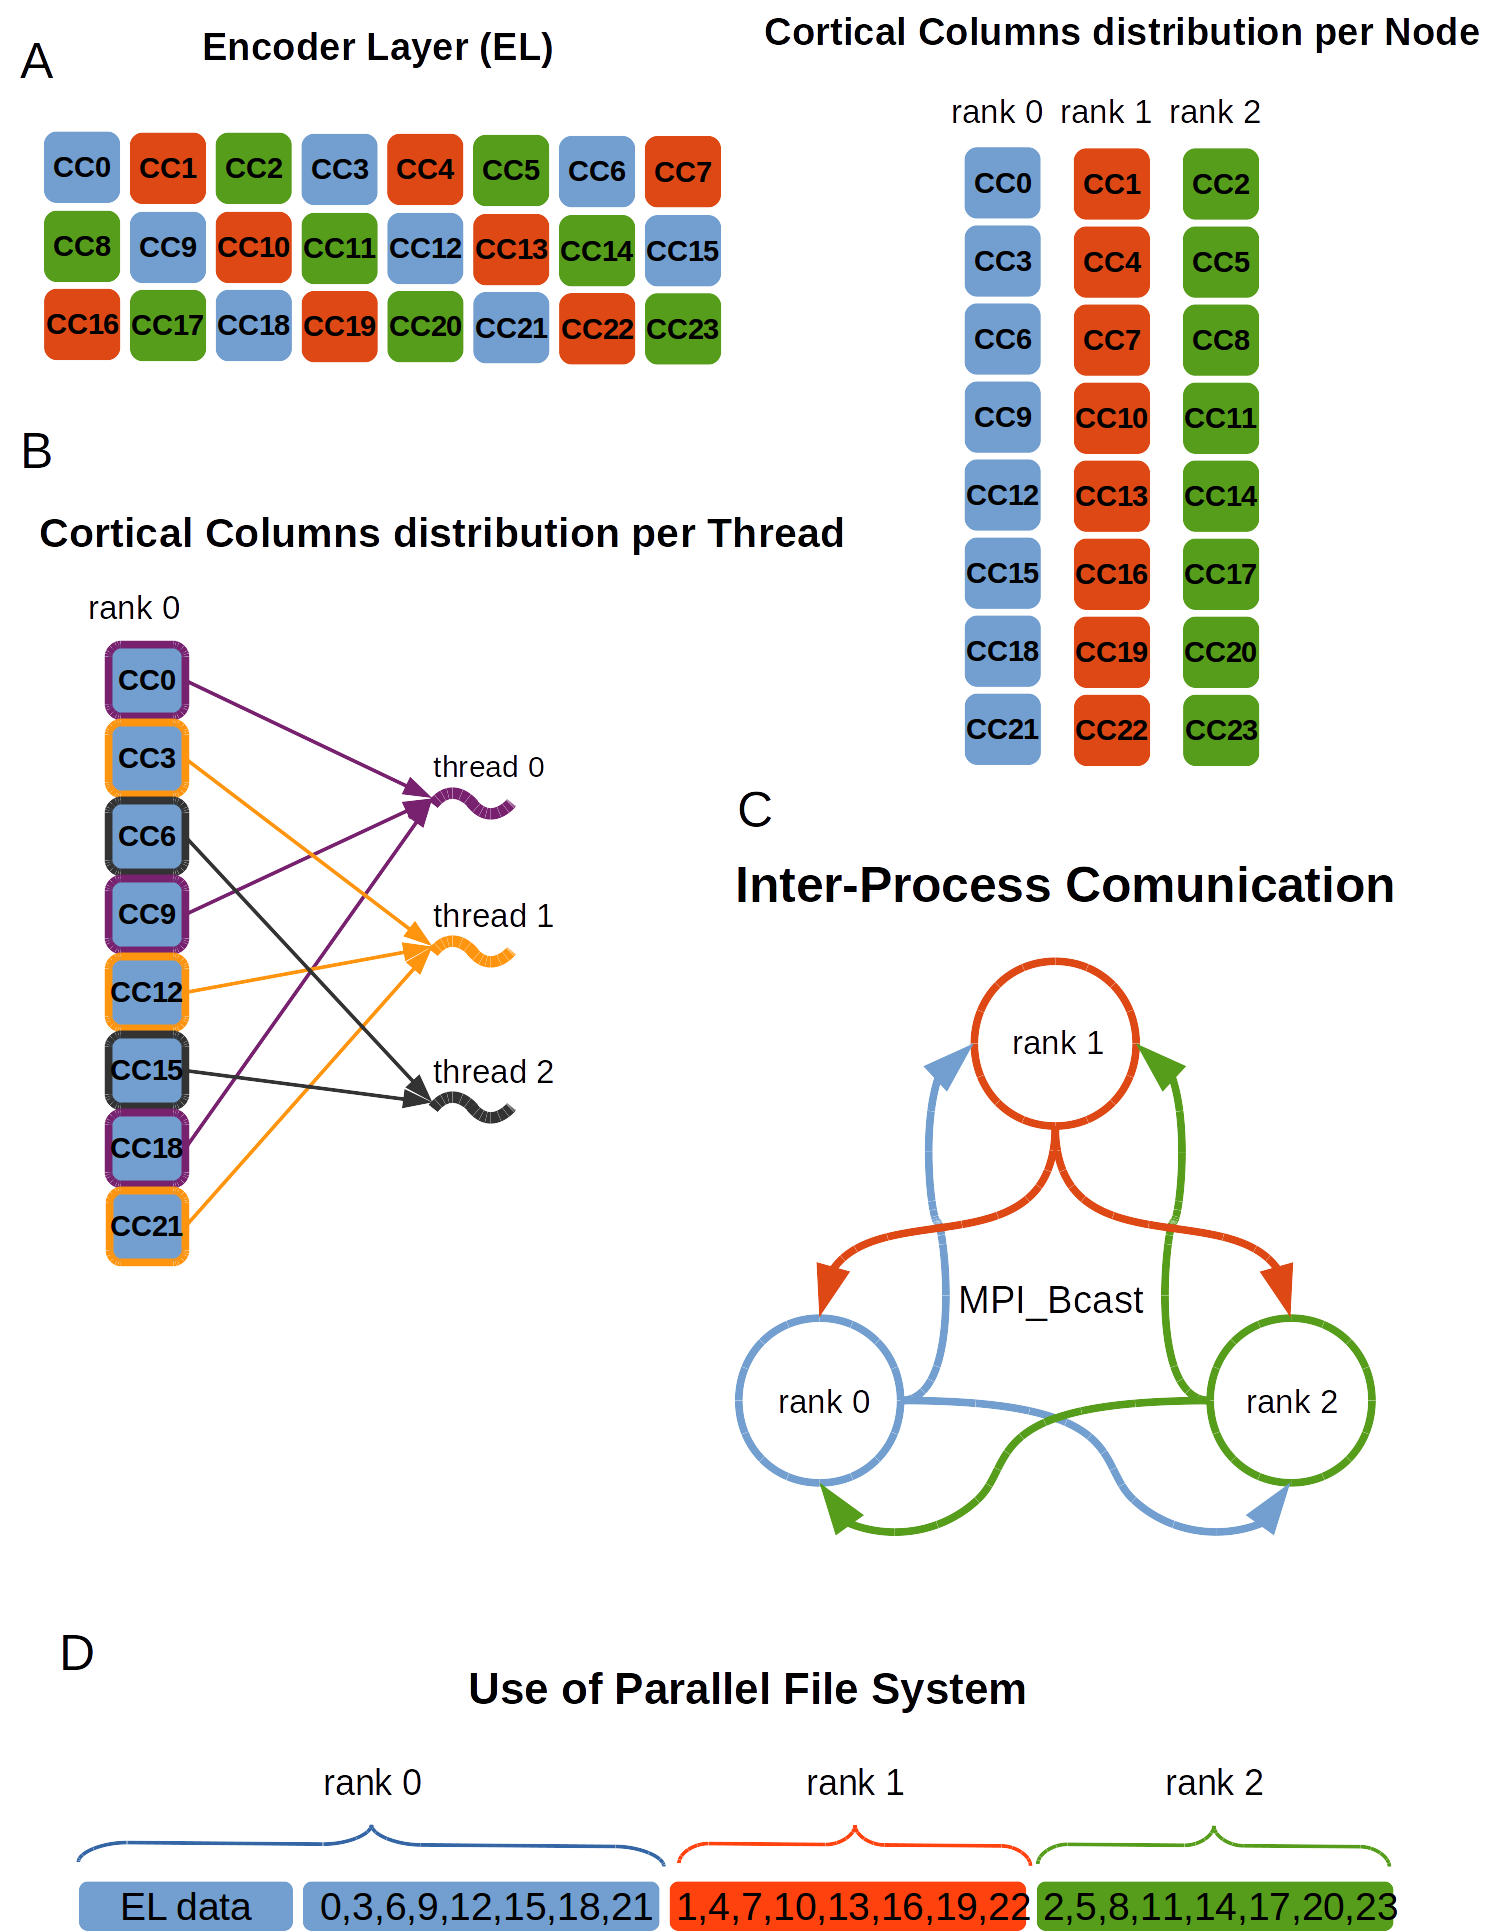
\includegraphics[width=0.7\textwidth]{EncoderParallelization.png}
    \caption{Paralelización \gls{mpi}+\gls{omp} del \glsfirst{el}. (A) Distribución de objetos \gls{csom} en un \gls{el} con
	    3 por 8 (24) \glspl{cc} entre tres \gls{mpi} ranks con tres hilos \gls{omp} por rank.
    Ciertos ranks podrían hacerse cargo de un número diferente de
    \glspl{csom} dependiendo del número de \gls{mpi} ranks así como también del número de \glspl{cc} en el \gls{el}.
    (B) Cada \gls{mpi} rank distribuye sus \glspl{csom} entre diferentes hilos de la misma manera.
    (C) \gls{mpi} \gls{ipc} entre diferentes ranks. El \gls{ipc} se lleva a cabo en cada paso temporal ya que cada \gls{mpi} rank 
    requiere la salida completa del \gls{el} en cada paso temporal.
    Cada \gls{mpi} rank difunde la información correspondiente a sus \glspl{cc} a los otros ranks en el ambiente \gls{mpi}.
    (D) Distribución de la información del \gls{el} en un archivo para guardar su estado.
    Cada \gls{mpi} rank pone los datos formateados correspondientes a sus \glspl{csom} en una clase template \gls{stl} stringstream.
    El Rank 0 también se hace cargo de la estructura, conectividad y parámetros del \gls{el}.
    Una vez que cada rank tiene su stringstream con los datos formateados, comunica su file view a los otros ranks.
    Luego, cada rank escribe su flujo de bytes en paralelo sin interferir con los otros ranks en el ambiente \gls{mpi}.
    Un \gls{el} con un número diferente de ranks puede cargar el mismo archivo sin afectar el resultado final.
    Cada rank en el nuevo \gls{el} carga el archivo completo en una clase template \gls{stl} stringstream y luego toma la información que le concierne de tal estructura.}
    %\caption{\glsfirst{el} \gls{mpi}+\gls{omp} parallelization. (A) Distribution of \gls{csom} objects in an \gls{el} with
    %3 by 8 (24) \glspl{cc} among three \gls{mpi} ranks with three \gls{omp} threads per rank.
    %Certain ranks could take care of a different number of
    %\glspl{csom} depending on the number of \gls{mpi} ranks as well as the number of \glspl{cc} in the \gls{el}.
    %(B) Each \gls{mpi} rank distributes its \glspl{csom} among different threads in the same fashion.
    %(C) \gls{mpi} \gls{ipc} among different ranks. \gls{ipc} is carried out at each time step since each \gls{mpi} rank 
    %requires the complete \gls{el} output at each time step.
    %Each \gls{mpi} rank broadcasts the information corresponding to its \glspl{cc} to the other ranks in the \gls{mpi}
    %environment.
    %(D) \gls{el} information distribution in a file to save its status.
    %Each \gls{mpi} rank puts the formated data corresponding to its \glspl{csom} in a \gls{stl} stringstream class template.
    %Rank 0 also takes care of the \gls{el} structure, connectivity and parameters.
    %Once each rank has its stringstream with the formated data, it communicates its file view to the other ranks.
    %Then each rank writes its stream of bytes in parallel without interfering with other ranks in the \gls{mpi} environment.
    %An \gls{el} with a different number of ranks can load the same file without affecting the final results.
    %Each rank in the new \gls{el} loads the complete file in a \gls{stl} stringstream class template and then takes the
    %informations that concern it from such structure.}
    \label{fig:EncoderParallelization}
\end{figure}



\subsection{Proceso Inicial de Pruebas de Strong y Weak Scaling en Cooley}

Más allá del hecho de que nuestra aplicación computacional está destinada a ser corrida en recursos computacionales de alto desempeño en el futuro, en el presente trabajo consideramos de esencial importancia poner bajo prueba nuestro código para poder juzgar cómo este utiliza los recursos computacionales provistos por los nodos de Cooley. La escalabilidad paralela es una medida que indica cuan eficiente es nuestro código a la hora de utilizar un número progresivamente creciente de elementos paralelos de procesamiento--ya sea Nodos o Procesos y \glspl{cpu} o Hilos en Cooley.

%Beyond the fact that our computational approach is intended to be applied in leadership supercomputers in the future, in the present work an essential step is to test our code in order to see how it uses the resources provided by Cooley Nodes. Parallel scalability is a measurement that indicates how efficient is our code when using increasing numbers of parallel processing elements --Nodes or Processes and \glspl{cpu} or Threads on Cooley.

La Fig. \ref{fig:Strong_Weak} muestra la capacidad de escalamiento de nuestro código en términos de tiempo vs. número de elementos de procesamiento utilizados para la tarea. En estas pruebas siempre restringimos nuestro código para que corriera un rank (proceso) \gls{mpi} por cada nodo en Cooley. Cada rank \gls{mpi} lanza un número de hilos específico y los reparte en los diferentes \glspl{cpu} en un nodo correspondiente (Fig. \ref{fig:EncoderParallelization} A y B). Hay dos maneras de medir desempeño paralelo en una aplicación dada. La medición que se aplique dependerá de si la aplicación está limitada en procesamiento o en memoria (\gls{cpu}-bound o memory-bound). Estas mediciones se llaman \emph{strong} y \emph{weak} scaling, respectivamente.

%Fig. \ref{fig:Strong_Weak} shows the scaling capacity of our code in terms of run time vs. number of processing elements used for the task. In our tests we always constrain our code to run one \gls{mpi} rank per Cooley node. Each \gls{mpi} rank spreads an specific number of threads through the different \glspl{cpu} in its corresponding node (Fig. \ref{fig:EncoderParallelization} A and B). There are two ways to measure the parallel performance of a given application. The measure to be applied will depend on whether the application is \gls{cpu}-bound or memory-bound. Such measurements are referred to as \emph{strong} and \emph{weak} scaling, respectively.



\begin{figure}[h!]
    \centering
    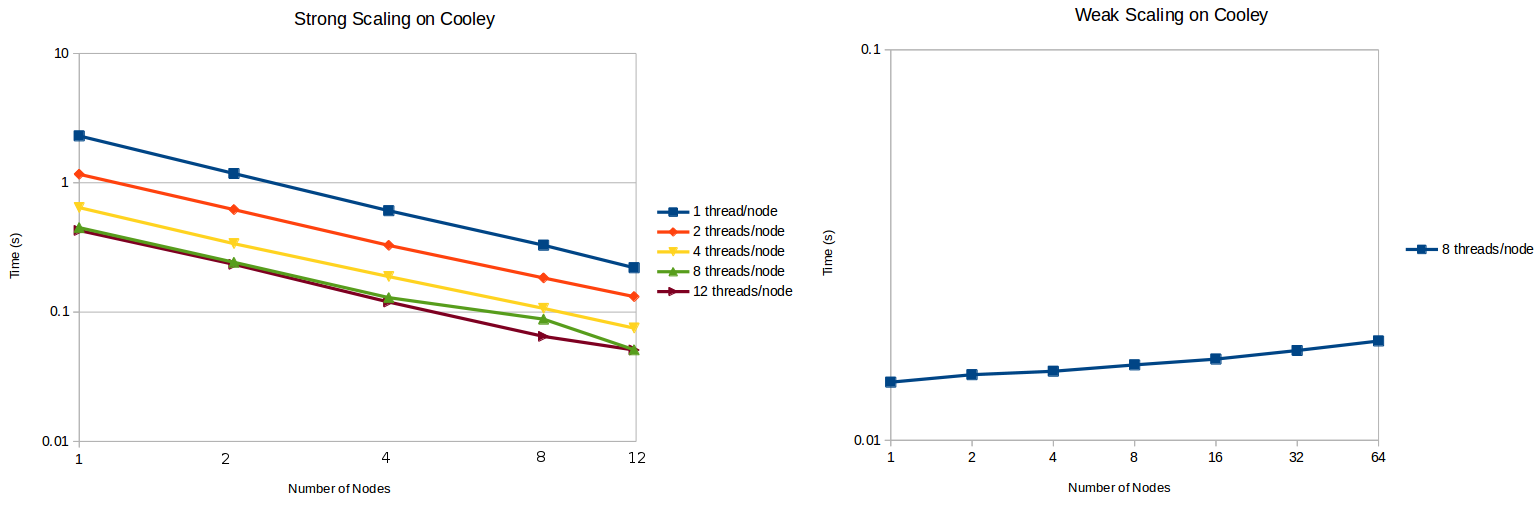
\includegraphics[width=1.0\textwidth]{Strong_Weak.png}
    \caption{Pruebas de Strong y Weak scaling en los nodos de Cooley. Izquierda: Strong scaling. Tiempo de corrida vs. el número de nodos para diferente número de hilos por nodo. El tamaño del problema a correr se mantiene fijo pero el número de elementos de procesamiento es incrementado. Derecha: Weak scaling. Tiempo de corrida vs. el número de nodos para 8 hilos por nodo. En este caso, la carga computacional del problema asignada a cada elemento de procesamiento se mantiene constante y se utilizan elementos adicionales para resolver problemas con cargas computacionales mayores.}
    %\caption{Strong and Weak scaling tests on Cooley nodes. Left: Strong scaling. Run time vs. the number of nodes for different number of threads per node. The problem size stays fixed but the number of processing elements are increased. Right: Weak scaling. Run time vs. the number of nodes for 8 threads per node. In this case the problem workload assigned to each processing element stays constant and additional elements are used to solve a larger total problem (i.e. a problem that would not fit in the available RAM on a single node).}
    \label{fig:Strong_Weak}
\end{figure}

Las líneas rectas en la Fig. \ref{fig:Strong_Weak} (izquierda) muestran una buena escalabilidad inicial de nuestro código en términos de \emph{Strong Scaling} mientras que la pequeña pendiente exhibida por la Fig. \ref{fig:Strong_Weak} (derecha) nos permite avisorar un buen desempeño en términos de \emph{Weak Scaling} de nuestro código para su implementación en supercomputadoras de gama alta en un futuro.

%Straight lines in Fig. \ref{fig:Strong_Weak} (left) show an initially good strong scalability of our code while the small slope exhibited by Fig. \ref{fig:Strong_Weak} (right) allows us to foresee a good weak scaling performance of our code in high end leadership supercomputers.

